\chapter{Acceso a carpetas}
\begin{center}
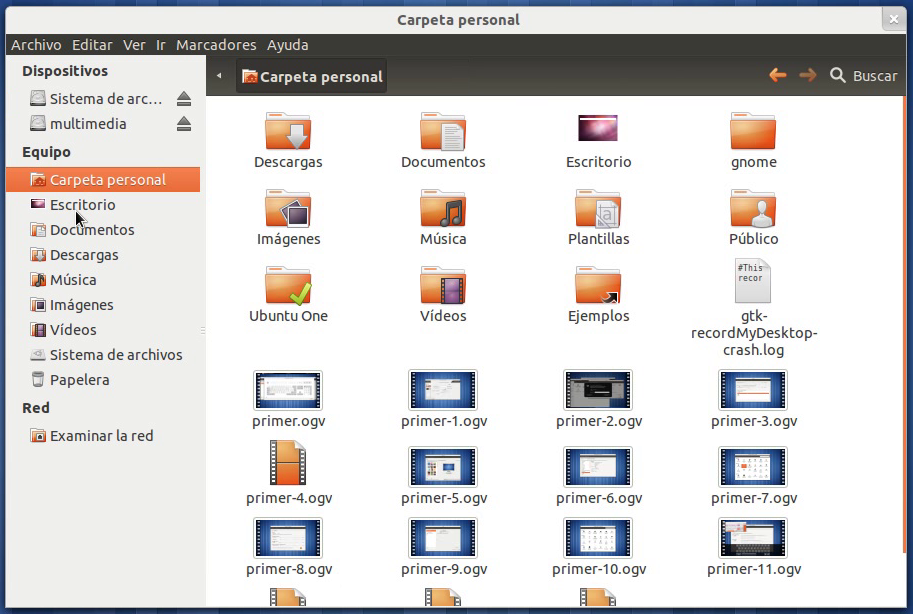
\includegraphics[scale=0.6]{gnome/carpetass.png}
\end{center}
Existen varios gestores de archivos en linux.
Nautilus, es el gestor gráfico de archivos de Gnome, muy fácil de usar.
\begin{itemize}
\item Tiene barra lateral, que se ve muy bien y permite organizar tus “lugares” de forma más sencilla y fácil para navegar por el árbol de directorios.
\item Incorpora una barra de herramientas novedosa e información inteligente de estado.
\item Puede conectarse a un servidor de archivos.
\end{itemize}
A continuación veremos las diferentes tareas de nautilus:
\section{Tareas comunes}
\subsubsection{Examinar archivos y carpetas}
Use la aplicación Archivos para navegar y organizar los archivos en su equipo. También puede usarlo para gestionar archivos en dispositivos de almacenamiento (como discos externos), en servidores de archivos y en recursos compartidos de la red.\\
Para abrir el gestor de archivos, entras en actividades. escribes nautilus y enter si te sale el gestor de archivos.\\
Para pulse acceder a cualquier carpeta pulsa dos veces sobre una carpeta para ver su contenido, o sobre un archivo para abrirlo con la aplicación predeterminada para ese archivo. También puede pulsar con el botón derecho sobre una carpeta para abrirla en una pestaña o una ventana nueva.\\ 
En la vista de lista, también puede pulsar en el extensor situado junto a la carpeta para mostrar su contenido en forma de árbol.\\
Al examinar los archivos en una carpeta puede previsualizar rápidamente cada archivo rápidamente pulsando la barra espaciadora para asegurarse de que tiene el archivo correcto antes de abrirlo, copiarlo o eliminarlo.\\
La barra de rutas situada encima de la lista de archivos y carpetas muestra qué carpeta esta visualizando, incluyendo sus carpetas padre hasta su carpeta personal. Pulse en una carpeta padre de la barra de rutas para moverse a esa carpeta. Pulse con el botón derecho sobre cualquier carpeta de la barra de rutas para abrirla en una pestaña o ventana nueva, copiarla, moverla o acceder a sus propiedades.\\
Si quieres saltar rápidamente a un archivo en la carpeta que está viendo, empiece a escribir su nombre. Aparecerá una caja de búsqueda en la parte inferior de la ventana y se resaltará el primer archivo que coincida con su búsqueda. Pulse la flecha abajo , Ctrl+G o desplácese con el ratón para saltar al siguiente archivo que coincida con su búsqueda.\\
Puede acceder rápidamente a lugares comunes desde la barra lateral. Si no ve la barra lateral, pulse en Ver $>$ Barra lateral $>$ Mostrar barra lateral. Puede añadir marcadores a carpetas que use con frecuencia y aparecerán en la barra lateral. Use el menú Marcadores para hacer esto, o simplemente arrastre una carpeta a la barra lateral.\\
Si mueve frecuentemente archivos entre carpetas anidadas, puede encontrar útil mostrar un árbol en la barra lateral. Pulse Ver $>$ Barra lateral $>$ Árbol, para activar el árbol de la barra lateral. Pulse el expansor junto a la carpeta para mostrar sus carpetas hijas en el árbol, o pulse en una carpeta para abrirla en la ventana.
\subsubsection{Buscar archivos}
Puede buscar archivos según su nombre o su tipo de archivo directamente desde el gestor de archivos. También puede guardar búsquedas frecuentes, que aparecerán como carpetas especiales dentro de su carpeta personal.\\

{\large \bf Buscar}
\begin{enumerate}
\item Abra la aplicación Archivos desde la vista de Actividades.
\item Si sabe que los archivos que quiere buscar están en una carpeta determinada, vaya a esa carpeta.
\item Pulse Buscar en la barra de herramientas, o pulse Ctrl+F.
\item Teclee una o varias palabras que sepa que aparecen en el nombre del archivo y pulse Intro. Por ejemplo, si todas sus facturas contienen en su nombre la palabra Factura, teclee factura. Pulse Intro No hace falta tener en cuenta las mayúsculas y minúsculas.
\item Puede acotar los resultados por ubicación y tipo de archivo. Pulse el botón + para establecer más criterios de búsqueda.
\begin{itemize}
\item Para acotar los resultados de la búsqueda, seleccione Ubicación de la lista desplegaba para añadir una ubicación padre.
\item Para acotar los resultados de la búsqueda en función del tipo de archivo, seleccione Tipo de archivo de la lista desplegable.
Pulse el botón - junto a cualquier opción de búsqueda para quitar esa opción y aumentar los resultados de búsqueda.
\end{itemize}
\item Puede abrir, copiar, eliminar o trabajar con sus archivos desde los resultados de búsqueda, igual como si estuviera en cualquier carpeta en el gestor de archivos.
\item Pulse de nuevo Buscar en la barra de herramientas para salir de la búsqueda y volver a la carpeta.
\end{enumerate}
Si lleva a cabo ciertas búsquedas muy a menudo, puede guardarlas para acceder a ellas rápidamente.\\

{\large \bf Guardar una búsqueda}
\begin{enumerate}
\item Iniciar una búsqueda como la de arriba.
\item Cuando esté satisfecho con sus parámetros de búsqueda, pulse Archivo $>$ Guardar búsqueda como.
\item Asigne un nombre a la búsqueda y pulse Guardar. Si lo desea, seleccione una carpeta distinta en la que guardarla. Cuando visualice esa carpeta, verá sus búsquedas guardadas como un icono de carpeta color naranja con una lupa.
\end{enumerate}
Para eliminar el archivo buscado cuando haya terminado con él, simplemente elimínelo de la búsqueda igual que haría con cualquier otro archivo. Cuando elimina una búsqueda guardada, no elimina los archivos que coincidieron con la búsqueda.
\subsubsection{Copiar o mover archivos y carpetas}
Es posible copiar o mover un archivo o carpeta en una nueva ubicación arrastrando y soltando con el ratón, usando los comandos de copiar y pegar, o mediante combinaciones de teclas.\\

Por ejemplo, es posible que quiera copiar una presentación en una tarjeta de memoria para trabajar con ella. O bien, podría hacer una copia de seguridad de un documento antes de realizar cambios en el mismo (y luego utilizar la copia antigua no le gustan los cambios).\\
Estas instrucciones se aplican tanto a los archivos como a las carpetas. Copia y mueve archivos y carpetas de la misma forma.\\

{\bf Copiar y pegar archivos}\\
\begin{enumerate}
\item Seleccione el archivo que quiera copiar, pulsándolo una sola vez.
\item Pulse Editar $>$ Copiar, o Ctrl+C.
\item Vaya a otra carpeta donde quiera poner la copia del archivo.
\item Pulse Editar $>$ Pegar para finalizar la copia del archivo, o pulse Ctrl+V. Ahora habrá una copia del archivo en la carpeta original y en la otra carpeta.
\end{enumerate}

{\bf Cortar y pegar archivos para moverlos}\\
\begin{enumerate}
\item Seleccione el archivo que quiere mover pulsándolo una sola vez.
\item Pulse Editar $>$ Cortar, o Ctrl+X.
\item Vaya a otra carpeta donde quiera mover el archivo.
\item Pulse Editar $>$ Pegar para finalizar el movimiento del elemento o pulse Ctrl+V. El archivo se tomará de su carpeta original y se moverá a la otra carpeta.
\end{enumerate}

{\bf Arrastrar archivos para copiarlos o moverlos}
\begin{enumerate}
\item Abra el gestor de archivos y vaya a la carpeta que contenga el elemento que quiere copiar.
\item Pulse Archivo $>$ Ventana nueva (o pulse Ctrl+N) para abrir una segunda ventana. En la ventana nueva, navegue hasta la carpeta donde quiere copiar o mover el elemento.
\item Pulse y arrastre el elemento de una ventana a la otra. Esto lo moverá si el destino está en el mismo dispositivo, o lo copiará si el destino está en un dispositivo diferente.
\item Por ejemplo, si arrastra un archivo de una memoria USB a su carpeta personal éste se copiará porque lo está arrastrando desde un dispositivo a otro.
\item Para forzar a que se copie el archivo manteniendo pulsada la tecla Ctrl mientras arrastra el archivo, o forzar mover el archivo manteniendo pulsada la tecla Mayús. mientras arrastra el archivo.
\end{enumerate}
Puede pulsar F3 en el gestor de carpetas para obtener una nuevo navegador de carpetas donde podrás realizar todas las mismas operaciones.\\

No puede copiar o mover un archivo en una carpeta de solo lectura. Algunas carpetas son de solo lectura para impedir que pueda hacer cambios en su contenido. Puede hacer que deje de ser de solo lectura
\subsubsection{Eliminar archivos y carpetas}
Si ya no quiere un archivo o carpeta, puede eliminarlo.\\
Cuando elimina un elemento, este se mueve a la carpeta Papelera, donde queda almacenado hasta que vacíe la papelera. Los elementos almacenados en la carpeta Papelera se pueden restaurar a su ubicación original si decide que los necesita, o si se eliminaron accidentalmente.
\begin{enumerate}
\item  Seleccione el elemento que quiere eliminar pulsándolo una sola vez.
\item Pulse Ctrl+Del en su teclado. Alternativamente, arrastre el elemento hasta la Papelera en la barra lateral.
\end{enumerate}
Para eliminar archivos de forma permanente y liberar espacio de disco en su equipo, debe vaciar la papelera. Para vaciar la papelera, pulse con el botón derecho en la Papelera en la barra lateral y seleccione Vaciar la papelera. También puede eliminar elementos individuales de la papelera examinando la misma desde la barra lateral o el menú Ir. Seleccione los archivos que quiere eliminar permanentemente y pulse Ctrl+Supr en su teclado, o pulse con el botón derecho y seleccione \underline{Eliminar permanentemente}.\\

Los archivos eliminados en dispositivos extraíbles puede no ser visibles en otros sistemas operativos, tales como Windows o Mac OS. Los archivos siguen ahí, y estarán disponibles cuando conecte el dispositivo de nuevo en su equipo.\\

{\bf Eliminar permanentemente un archivo}\\
Puede eliminar un archivo permanentemente de forma inmediata, sin tenerlo que enviar primero a la papelera.
\begin{enumerate}
\item Seleccione el elemento que quiere eliminar.
\item Pulse y mantenga pulsada la tecla Mayús, y luego pulse la tecla Supr de su teclado.
\item Como no puede deshacer esta operación, se le preguntará que confirme si quiere eliminar el archivo o carpeta.
\end{enumerate}
Si necesita con frecuencia eliminar archivos sin usar la papelera (por ejemplo, si trabaja a menudo con datos sensibles), puede añadir una opción Eliminar al menú contextual de archivos y carpetas. Pulse Editar $>$ Preferencias y seleccione la pestaña Comportamiento. Seleccione Incluir el comando \underline{Eliminar} que no use la papelera.
\subsubsection{Ordenar archivos y carpetas}
Puede ordenar los archivos de una carpeta de diferentes formas; por ejemplo, por fecha o tamaño. Consulte la Maneras de ordenar archivos a continuación una lista de formas habituales de ordenar archivos.\\
Cuando cambia la manera de ordenar elementos en una carpeta, solo afecta a esa carpeta. El gestor de archivos recordará sus preferencias de ordenación para esa carpeta, pero usará el criterio de ordenación predeterminado en las demás carpetas. Consulte la Preferencias de las vistas del gestor de archivos para obtener más información sobre cómo cambiar el criterio de ordenación predeterminado.\\
La forma en la que ordene los archivos dependerá de la vista de carpeta que esté usando. Puede cambiar la vista actual usando el menú Ver.
\begin{itemize}
\item {\bf Vista de icono}\\
Para ordenar los archivos de forma diferente, pulse con el botón derecho en un lugar vacío de la carpeta y seleccione una opción del menú Organizar los elementos. También puede usar el menú Ver $>$ Organizar los elementos.\\
Por ejemplo, si selecciona Ordenar por nombre en el menú Organizar los elementos, los archivos se ordenarán según sus nombres. Consulte otras opciones en la Maneras de ordenar archivos.\\

Puede ordenar en orden inverso seleccionando Orden inverso en el menú Organizar los elementos.\\
Para controlar totalmente el orden y la posición de los archivos en la carpeta, pulse con el botón derecho en un lugar vacío de la carpeta y seleccione Organizar los elementos $>$ Manualmente. Así podrá reorganizar los archivos arrastrándolos y soltándolos por la carpeta. La ordenación manual solo funciona en la vista de iconos.\\
La opción Disposición compacta del menú Organizar los elementos organiza los archivos de forma que ocupan el menor espacio posible. Es útil si quiere ver un montón de archivos al mismo tiempo en una carpeta.
\item {\bf Vista de lista}\\ Para ordenar los archivos de forma diferente, pulse en una de las cabeceras de las columnas en el gestor de archivos. Por ejemplo, pulse en Tipo para ordenar por tipo de archivo. Pulse de nuevo en la cabecera de la columna para ordenar en orden inverso.\\
En la vista de lista, puede mostrar las columnas con más atributos y ordenar estas columnas. Pulse en Vista $>$ Columnas visibles y seleccione las columnas que desea que sean visible. A continuación, podrá ordenar por esas columnas. Consulte la Preferencias de las columnas en la lista del gestor de archivos para obtener las descripciones de las columnas disponibles.
\item {\bf Vista compacta}\\ Puede ordenar los archivos en la vista compacta de la misma manera que puede ordenar la vista de iconos. La única diferencia es que no se puede colocar manualmente los archivos en cualquier lugar que desee, siempre están organizados en una lista en esta vista.
\item {\bf Maneras de ordenar archivos}\\
\begin{itemize}
\item {\bf Por nombre.-} Ordena alfabéticamente por el nombre del archivo.
\item {\bf Por tamaño.-} Ordena por el tamaño del archivo (cuánto espacio ocupa). Ordena de menor a mayor de manera predeterminada.
\item {\bf Por tipo.-} Ordena alfabéticamente por el tipo de archivo. Los archivos del mismo tipo se agrupan, a continuación, ordenados por nombre.
\item {\bf Por fecha de modificación.-} Ordena por la fecha y hora en las que se modificó un archivo por última vez. Ordena de la más antigua a la más reciente de manera predeterminada.
\end{itemize}
\end{itemize}
\subsubsection{Previsualizar archivos y carpetas}
Puede previsualizar archivos rápidamente sin abrirlos en una aplicación completa. Seleccione un archivo y pulse la barra espaciadora. El archivo se abrirá en una ventana simple de vista previa. Pulse la barra espaciadora de nuevo para cerrar la vista previa.\\
La vista previa soporta la mayoría de formatos de archivo para documentos, imágenes, vídeo y sonido. En la vista previa puede desplazarse por sus documentos o buscar a través de sus vídeos y archivos de sonido.\\
Para ver una vista previa a pantalla completa, pulse el botón f. o pulse la barra espaciadora.
\subsubsection{Renombrar un archivo o una carpeta}
Puede cambiar el nombre de un archivo o de una carpeta.
\begin{enumerate}
\item Pulse con el botón derecho sobre un archivo o carpeta y seleccione Renombrar, o seleccione el archivo y pulse F2.
\item Escriba el nombre nuevo y pulse Intro.
\end{enumerate}
También puede renombrar un archivo desde la ventana de propiedades.\\
Cuando cambia el nombre de un archivo, solo se selecciona la primera parte del nombre de ese archivo, sin la extensión (la parte que va detrás del punto “.”). La extensión normalmente representa el tipo de archivo (p.ej archivo.pdf es un documento PDF), y normalmente no querrá cambiarla. Si necesita cambiar la extensión también, seleccione el nombre completo del archivo y cámbielo.\\

{\bf Problemas comunes}
\begin{itemize}
\item {\bf El nombre ya está en uso}\\
No puede tener dos archivos o carpetas con el mismo nombre en la misma carpeta. Si al cambiar el nombre a un archivo intenta asignarle uno que ya existe en la carpeta donde está trabajando, el gestor de archivos no se lo permitirá. Use un nombre distinto.\\
Los nombres de archivos y carpetas distinguen las mayúsculas y las minúsculas. Por ejemplo, Archivo.txt y archivo.txt son dos nombres diferentes. Esto esta permitido, aunque no siempre es una buena idea.\\
\item {\bf El nombre de archivo demasiado largo}\\
En algunos sistemas de archivos, los nombres de archivos no pueden contener más de 255 caracteres. Use un nombre más corto.
\item {\bf La opción para renombrar está en gris}\\
Si la opción Renombrar aparece en color gris, es que no tiene los permisos necesarios para cambiar el nombre del archivo. Normalmente, si no tiene los permisos adecuados, no debería intentar renombrarlo. Consulte la Establecer los permisos del archivo.
\end{itemize}
\section{Otros temas}
\subsubsection{Abrir archivos con otras aplicaciones}
Cuando se pulsa dos veces sobre un archivo en el gestor de archivos, se abre con la aplicación predeterminada para ese tipo de archivos. Puede abrirlo con una aplicación distinta, buscar aplicaciones en línea, o establecer la aplicación predeterminada para todos los archivos del mismo tipo.\\

Para abrir un archivo con una aplicación distinta de la predeterminada, pulse en el archivo y seleccione la aplicación que desee en la parte superior del menú. Si no ve la aplicación que quiere, pulse en Abrir con otra aplicación. De manera predeterminada, el gestor de archivos solo muestra las aplicaciones que sabe que pueden manejar el archivo. Para buscar todas las aplicaciones en su equipo, pulse en Mostrar otras aplicaciones.\\
Si aun no encuentra la aplicación que quiere, puede buscar más aplicaciones pulsando Buscar aplicaciones en línea. El gestor de archivos buscará en línea paquetes que contengan aplicaciones que manejen archivos de ese tipo.\\

{\bf Cambiar la aplicación predeterminada}\\
Puede cambiar la aplicación predeterminada usada para abrir los archivos de un cierto tipo. Esto le permitirá abrir su aplicación preferida cuando pulse dos veces sobre un archivo para abrirlo. Por ejemplo, puede que quiera que se abra su reproductor de música favorito al pulsar dos veces sobre un archivo MP3.
\begin{enumerate}
\item Seleccione un archivo del tipo cuya aplicación predeterminada desea cambiar. Por ejemplo, para cambiar la aplicación usada para abrir archivos MP3, seleccione un archivo .mp3.
\item Pulse con el botón derecho del ratón y seleccione Propiedades.
\item Seleccione la pestaña Abrir con.
\item Seleccione la aplicación que quiere y pulse Establecer como predeterminada. De manera predeterminada, el gestor de archivos solo muestra aplicaciones que sabe que pueden manejar el archivo. Para buscar entre todas las aplicaciones en su equipo, pulse Mostrar otras aplicaciones.
\end{enumerate}
Si \underline{Otras aplicaciones} contiene una aplicación que desea usar a veces, pero que no quiere convertir en la predeterminada, seleccione esa aplicación y pulse en Añadir. Esto la añadirá a Aplicaciones recomendadas. A partir de entonces podrá usar la aplicación pulsando con el botón derecho sobre el archivo y seleccionándola de la lista.\\

Esto cambiará la aplicación predeterminada no solo para el archivo seleccionado, sino para todos los archivos del mismo tipo.
\subsubsection{Compartir y transferir archivos}
Puede compartir archivos fácilmente con sus contactos o transferirlos a dispositivos externos o a recursos compartidos de la red directamente desde el gestor de archivos.\\
\begin{itemize}
\item Abra la aplicación Archivos desde la vista de Actividades.
\item Seleccione el archivo que quiere transferir.
\item Pulse con el botón derecho del ratón y seleccione Enviar a....
\item Aparecerá la ventana Enviar a. Seleccione a dónde desea enviar el archivo y pulse Enviar.\\ Para obtener más información, consulte la siguiente lista de destinos.
\end{itemize}
Puede enviar varios archivos a la vez. Seleccione varios archivos manteniendo pulsada la tecla Ctrl y pulse con el botón derecho sobre cualquier archivo seleccionado. Podrá comprimir los archivos automáticamente en un archivador tar o zip.\\

{\bf Destinos}\\
\begin{itemize}
\item Para enviar por correo electrónico el archivo, seleccione Correo-e e introduzca la dirección del correo electrónico del destinatario.
\item Para enviar el archivo a un contacto de mensajería instantánea, seleccione Mensaje instantáneo, y seleccione el contacto en la lista desplegable. Para que funcione, es posible que tenga que iniciar su programa de mensajería instantánea.
\item Para grabar el archivo en un CD o DVD, seleccione Creador de CD/DVD. Consulte la Escribir archivo en un CD o DVD para obtener más información.
\item Para transferir el archivo a un dispositivo Bluetooth, seleccione Bluetooth (OBEX Push) y seleccione el archivo al que enviarlo. Sólo verá dispositivos que ya estén emparejados Consulte la Bluetooth para obtener más información.
\item Para copiar el archivo a un dispositivo externo como una memoria flash USB, o subirlo a un servidor al que está conectado, seleccione Soportes extraíbles y comparticiones y a continuación seleccione el dispositivo o servidor en el que quiere copiar el archivo
\end{itemize}
\subsubsection{Encontrar un archivo perdido}
Si ha creado o descargado un archivo, pero no sabe donde esta, siga estas indicaciones.\\
\begin{itemize}
\item Si no recuerda donde guardo el archivo, pero tiene cierta idea de como se llama, puede buscarlo por su nombre. Consulte la Buscar archivos para saber cómo.
\item Si acaba de descargar el archivo, su navegador web podría haberlo guardado automáticamente en una carpeta común. Compruebe las carpetas Escritorio y Descargas en su carpeta personal.
\item Es posible que haya eliminado el archivo accidentalmente. Cuando elimina un archivo, se mueve a la papelera, donde permanecerá hasta que vacíe la papelera manualmente.\\ Consulte la Recuperar un archivo eliminado para saber cómo recuperar un archivo eliminado.
\item Puede que haya cambiado el nombre del archivo de forma que ahora quede oculto. Los archivos que empiezan por . o que acaban en $~$ están ocultos en el gestor de archivos. Pulse Ver $>$ Mostrar los archivos ocultos en el gestor de archivos. Consulte la Ocultar un archivo para obtener más información.
\end{itemize}
\subsubsection{Escribir archivo en un CD o DVD}
Puede poner archivos en un disco vacío usando el Creador de CD/DVD. La opción de crear un CD o un DVD aparecerá en el gestor de archivos tan pronto como introduzca un CD en su grabador de CD/DVD. El gestor de archivos le permite transferir archivos a otros equipos o realizar copias de respaldo poniendo archivos en un disco vacío. Para escribir archivos en un CD o DVD
\begin{enumerate}
\item Coloque un disco vacío dentro de un unidad grabadora de CD/DVD.
\item En la ventana Disco CD/DVD-R vacío que aparece, seleccione Creador de CD/DVD y pulse Aceptar. Se abrirá la ventana de la carpeta del creador de CD/DVD.\\
(También puede pulsar en Disco CD/DVD-R virgen bajo Dispositivos en la barra lateral del gestor de archivos.)
\item En el campo Nombre del disco teclee un nombre para el disco.
\item Arrastre o copie los archivos que quiera a la ventana.
\item Pulse Escribir en el disco.
\item En Seleccione un disco en el que grabar seleccione el disco vacío.\\
(También puede elegir $>$ Archivo de imagen. Esto pondrá los archivos en una imagen de disco, que se guardará en su equipo. Más tarde podrá grabar esa imagen en un disco vacío.)
\item Pulse en Propiedades si desea ajustar la velocidad de grabación, la ubicación de los archivos temporales y otras opciones. Las opciones predeterminadas deberían ser suficientes.
\item Pulse el botón Grabar para comenzar la grabación.\\
Si selecciona Grabar varias copias, se le pedirá que introduzca más discos.
\item Cuando se haya grabado el disco por completo, se expulsará automáticamente. Seleccione Hacer más copias o Cerrar para salir.
\end{enumerate}
{\bf Si el disco no se grabó correctamente}\\
A veces, los discos no se graban correctamente y no podrá ver los archivos que puso en el disco cuando lo introduzca en un equipo.\\
En este caso, pruebe a grabar de nuevo el disco usando una velocidad de grabación más lenta; por ejemplo 12x en lugar de 48x. Grabar a velocidades más lentas es más fiable. También puede seleccionar la velocidad pulsando en el botón Propiedades de la ventana Carpeta del creador de CD/DVD.
\subsubsection{Examinar archivos en un servidor o compartición de red}
Puede conectarse a un servidor o a un recurso compartido para buscar y ver los archivos en el servidor, exactamente como si estuvieran en su máquina local o dispositivo extraíble. Esta es una manera conveniente para descargar o subir archivos, o para compartir archivos con usuarios en su red local.\\
Para examinar archivos en la red abra la aplicación de Archivos desde la vista general de Actividades. Después pulse Navegar por la red en la barra lateral, o seleccione Red en el menú Ir. El gestor de archivos buscará cualquier equipo en su red local que informe que puede servir archivos. Si quiere conectarse a un servidor de Internet, o si no ve el equipo que está buscando, puede conectarse manualmente a un servidor introduciendo su dirección de red o internet.\\

{\bf Conectar con un servidor de archivos}\\
\begin{enumerate}
\item En el gestor de archivos pulse Archivo $>$ Conectar con el servidor.
\item Introduzca la dirección del servidor, seleccione el tipo de servidor y escriba cualquier información adicional cuando se le solicite. Después, pulse en Conectar. Se listan debajo detalles acerca de los tipos de servidores.\\
Para servidores en Internet, generalmente se puede usar el nombre de dominio (ej. ftp.ejemplo.com). Sin embargo, para los equipos de su red de área local, puede que tenga que usar la dirección IP numérica del equipo.
\item Se abrirá una nueva ventana mostrando los archivos en el servidor. Puede examinar los archivos de igual forma que si estuviesen en su mismo equipo.\\

El servidor también se añadirá a la barra lateral para que pueda acceder rápidamente a él en el futuro
\end{enumerate}
{\bf Diferentes tipos de servidores}\\
Puede conectarse a diferentes tipos de servidores. Algunos servidores son públicos, y permiten a cualquiera conectarse. Otros servidores requieren que inicie sesión con su nombre de usuario y contraseña.\\
Puede que no tenga permisos para realizar ciertas acciones sobre los archivos en un servidor. Por ejemplo, en sitios FTP públicos, probablemente no podrá eliminar archivos.\\

{\bf Tipos de servidores}
\begin{itemize}
\item {\bf SSH}\\
Si tiene una cuenta SSH en un servidor, podrá conectarse usando este método. Muchos servidores de alojamiento web proporcionan cuentas SSH a sus miembros para que puedan subir archivos de forma segura. Los servidores SSH siempre requieren que usted inicie una sesión. Si usa una clave de SSH para iniciar sesión, deje el campo de contraseña en blanco.\\
Cuando se usa SSH, todos los datos que envía (incluyendo su contraseña) van cifrados, por lo que otros usuarios de su red no podrán verlos.
\item {\bf FTP (con registro)}\\
FTP es un protocolo muy popular para intercambiar archivos por Internet. Dado que los datos no están cifrados a través de FTP, muchos servidores ahora facilitan el acceso a través de SSH. Algunos servidores, sin embargo, todavía permiten o requieren el uso de FTP para subir o descargar archivos. Los sitios FTP con inicio de sesión generalmente le permitirán eliminar y subir archivos.
\item {\bf FTP público}\\
Los sitios que le permiten descargar archivos a veces proporcionan acceso FTP público o anónimo. Estos servidores no requieren un nombre de usuario y contraseña, y por lo general no le permiten eliminar o subir archivos.\\
Algunos sitios FTP anónimos requieren iniciar sesión con un nombre de usuario y contraseña pública, o con un nombre de usuario público utilizando su dirección de correo electrónico como contraseña. Para estos servidores, utilice el método de FTP (con entrada), y use las credenciales especificadas por el sitio FTP.
\item {\bf Compartición Windows}\\
Los equipos Windows usan un protocolo privativo para compartir archivos a través de una red de área local. Los equipos de una red Windows a veces se agrupan en dominios para organizar y controlar mejor el acceso. Si tiene los permisos adecuados en el equipo remoto, podrá conectarse a un recurso compartido de Windows desde el gestor de archivos.
\item {\bf WebDAV y WebDAV seguro}\\
Basado en el protocolo HTTP usado en la web, a veces se usa WebDAV para compartir archivos en una red local o guardarlos en Internet. Si el servidor al que se esta conectando admite conexiones seguras, debería escoger esta opción. WebDAV seguro usa cifrado SSL fuerte, por lo que nadie podrá ver su contraseña ni sus datos.
\end{itemize}
\subsubsection{Propiedades del archivo}
Puede ver información sobre un archivo o carpeta, pulse con el botón derecho y seleccione Propiedades. También puede seleccionar el archivo y pulsar Alt+Intro.\\

La ventana de propiedades del archivo le muestra información tal como el tipo de archivo, su tamaño y cuándo lo modificó por última vez. Si necesita esta información a menudo, puede mostrarla en las columnas de la vista de lista o en las leyendas de los iconos.\\
La información básica dada en la pestaña Básico se explica a continuación. También están las pestañas Permisos y Abrir con. Para ciertos tipos de archivos, como imágenes y vídeos, habrá una pestaña adicional que proporcione información sobre el tamaño, la duración y el codec.\\

{\bf Propiedades básicas}
\begin{itemize}
\item {\bf Nombre}\\
Puede cambiar el nombre del archivo cambiando este campo. También puede cambiar el nombre de un archivo fuera de la ventana de propiedades. Consulte la Renombrar un archivo o una carpeta.
\item {\bf Tipo}\\
El tipo de un archivo, como documento PDF, texto de OpenDocument o imagen JPEG. El tipo MIME del archivo determina qué aplicaciones pueden abrir el archivo, entre otras cosas.Por ejemplo, no puede abrir una imagen con un reproductor de música. Consulte la Abrir archivos con otras aplicaciones para obtener más información.\\
Entre paréntesis se muestra el tipo MIME del archivo; el tipo MIME es una forma estándar que los equipos usan para referirse al tipo de archivo.
\item {\bf Contenido}\\
Este campo se muestra si está consultando las propiedades de una carpeta. Muestra el número de elementos de la carpeta. Si la carpeta incluye otras carpetas, cada carpeta interna se cuenta como un elemento, aunque contenga a su vez otros elementos. Cada archivo se cuenta como un elemento. Si la carpeta está vacía, el contenido no mostrará nada.
\item {\bf Tamaño}\\
Este campo se muestra si está viendo un archivo (no una carpeta). el tamaño de un archivo le indica cuanto espacio ocupa en el disco. También es un indicador de cuánto tardará en descargar un archivo o en enviarlo por correo-e (cuanto más grande es el archivo, más tarda al enviarse/recibirse).\\
Los tamaños se puede dar en bytes, KBs, MBs o GBs; en los tres últimos casos, el tamaño en bytes aparece entre paréntesis. Técnicamente, 1Kb son 1024 bytes, 1MB son 1024 KB, y así sucesivamente.
\item {\bf Ubicación}\\
La ubicación de cada archivo en su sistema viene dada por su ruta absoluta. Esto es una dirección única del archivo en el equipo, compuesta de una lista de carpetas a las que debe ir para encontrar el archivo. Por ejemplo, si Jaime tiene un archivo Resumen.pdf en su carpeta personal, la ubicación será /home/jaime/Resumen.pdf.
\item {\bf Volumen}\\
El sistema de archivo o el dispositivo en el que está almacenado el archivo. Esto le muestra dónde está almacenado físicamente el archivo, por ejemplo, si está en el disco duro, en un CD o en una carpeta de red o un servidor de archivos. Los discos duros se pueden dividir en varias particiones; la partición se mostrará también debajo del Volumen.
\item {\bf Espacio libre}\\
Esto sólo se muestra para las carpetas. Indica la cantidad total de espacio disponible en el disco en el que se encuentra la carpeta. Es útil para comprobar si el disco duro está lleno.
\item {\bf Accedido}\\
Fecha y hora de la última apertura del archivo.
\item {\bf Modificado}\\
Fecha y hora de la última vez que se cambió y guardó el archivo.
\end{itemize}
\subsubsection{Recuperar un archivo eliminado}
Si ha eliminado un archivo pulsando Ctrl+Supr, pulsando el elemento de menú Mover a la papelera o arrastrando el archivo a la papelera, el archivo debería estar en la papelera.\\

{\bf Restaurar desde la papelera}
\begin{enumerate}
\item Abra la aplicación Archivos desde la vista de Actividades.
\item Pulse Papelera en la barra lateral.
\item Si su archivo eliminado está ahí, pulse con el botón derecho sobre él y seleccione \underline{Restaurar}. Se devolverá a la carpeta de la que se borró
\end{enumerate}
Si eliminó el archivo usando Mayús+Eliminar o desde la línea de comandos, el archivo no se podrá recuperar usando este método porque se habrá eliminado permanentemente.\\
Existen varias herramientas de recuperación disponibles que a veces pueden recuperar archivos que se eliminaron permanentemente. No obstante, normalmente no son muy fáciles de usar. Si eliminó un archivo permanentemente de forma accidental, probablemente sea mejor pedir ayuda en los foros de soporte para ver si es posible recuperarlo.
%%\subsubsection{Preferencias del gestor de archivos}

